
% $Header: /cvsroot/latex-beamer/latex-beamer/solutions/generic-talks/generic-ornate-15min-45min.en.tex,v 1.5 2007/01/28 20:48:23 tantau Exp $

\documentclass[smaller]{beamer}
\mode<presentation>
{
  \usetheme{Singapore}
  \usefonttheme[onlymath]{serif}
  % or ...
 %  \setbeamercovered{transparent}
  % or whatever (possibly just delete it)
}


\usepackage[czech]{babel}
% or whatever
\usepackage[utf8]{inputenc}
% or whatever
%\usepackage{times}
%\usepackage[T1]{fontenc}
% Or whatever. Note that the encoding and the font should match. If T1
% does not look nice, try deleting the line with the fontenc.


\title{PAS02 - náhodné veličiny}

\author{Jan B\v rezina}
\institute % (optional, but mostly needed)
{
  %\inst{2}%
  Technical University of Liberec
}


% If you wish to uncover everything in a step-wise fashion, uncomment
% the following command: 

%\beamerdefaultoverlayspecification{<+->}

% ***************************************** SYMBOLS
\def\div{{\rm div}}
\def\Lapl{\Delta}
\def\grad{\nabla}
\def\supp{{\rm supp}}
\def\dist{{\rm dist}}
%\def\chset{\mathbbm{1}}
\def\chset{1}

\def\Tr{{\rm Tr}}
\def\sgn{{\rm sgn}}
\def\to{\rightarrow}
\def\weakto{\rightharpoonup}
\def\imbed{\hookrightarrow}
\def\cimbed{\subset\subset}
\def\range{{\mathcal R}}
\def\leprox{\lesssim}
\def\argdot{{\hspace{0.18em}\cdot\hspace{0.18em}}}
\def\Distr{{\mathcal D}}
\def\calK{{\mathcal K}}
\def\FromTo{|\rightarrow}
\def\convol{\star}
\def\impl{\Rightarrow}
\DeclareMathOperator*{\esslim}{esslim}
\DeclareMathOperator*{\esssup}{ess\,sup}
\DeclareMathOperator{\ess}{ess}
\DeclareMathOperator{\osc}{osc}
\DeclareMathOperator{\curl}{curl}

%\def\Ess{{\rm ess}}
%\def\Exp{{\rm exp}}
%\def\Implies{\Longrightarrow}
%\def\Equiv{\Longleftrightarrow}
% ****************************************** GENERAL MATH NOTATION
\def\Real{{\rm\bf R}}
\def\Rd{{{\rm\bf R}^{\rm 3}}}
\def\RN{{{\rm\bf R}^N}}
\def\D{{\mathbb D}}
\def\Nnum{{\mathbb N}}
\def\Measures{{\mathcal M}}
\def\d{\,{\rm d}}               % differential
\def\sdodt{\genfrac{}{}{}{1}{\rm d}{{\rm d}t}}
\def\dodt{\genfrac{}{}{}{}{\rm d}{{\rm d}t}}

\def\vc#1{\mathbf{\boldsymbol{#1}}}     % vector
\def\tn#1{{\mathbb{#1}}}    % tensor
\def\abs#1{\lvert#1\rvert}
\def\Abs#1{\bigl\lvert#1\bigr\rvert}
\def\bigabs#1{\bigl\lvert#1\bigr\rvert}
\def\Bigabs#1{\Big\lvert#1\Big\rvert}
\def\ABS#1{\left\lvert#1\right\rvert}
\def\norm#1{\bigl\Vert#1\bigr\Vert} %norm
\def\close#1{\overline{#1}}
\def\inter#1{#1^\circ}
\def\ol#1{\overline{#1}}
\def\ul#1{\underline{#1}}
\def\eqdef{\mathrel{\mathop:}=}     % defining equivalence
\def\where{\,|\,}                    % "where" separator in set's defs
\def\timeD#1{\dot{\overline{{#1}}}}

% ******************************************* USEFULL MACROS
\def\RomanEnum{\renewcommand{\labelenumi}{\rm (\roman{enumi})}}   % enumerate by roman numbers
\def\rf#1{(\ref{#1})}                                             % ref. shortcut
\def\prtl{\partial}                                        % partial deriv.
\def\Names#1{{\scshape #1}}
\def\rem#1{{\parskip=0cm\par!! {\sl\small #1} !!}}

\def\Xint#1{\mathchoice
{\XXint\displaystyle\textstyle{#1}}%
{\XXint\textstyle\scriptstyle{#1}}%
{\XXint\scriptstyle\scriptscriptstyle{#1}}%
{\XXint\scriptscriptstyle\scriptscriptstyle{#1}}%
\!\int}
\def\XXint#1#2#3{{\setbox0=\hbox{$#1{#2#3}{\int}$}
\vcenter{\hbox{$#2#3$}}\kern-.5\wd0}}
\def\ddashint{\Xint=}
\def\dashint{\Xint-}

% ******************************************* DOCUMENT NOTATIONS
% document specific
\def\rh{\varrho}
\def\vl{{\vc{u}}}
\def\th{\vartheta}
\def\vx{\vc{x}}
\def\vX{\vc{X}}
\def\vr{\vc{r}}
\def\veta{\vc{\eta}}
\def\dx{\,\d\vx}
\def\dt{\,\d t}
\def\bulk{\zeta}
\def\cS{\close{S}}
\def\eps{\varepsilon}
\def\phi{\varphi}
\def\Bog{{\mathcal B}}
\def\Riesz{{\mathcal R}}
\def\distr{\mathcal D}
\def\Item{$\bullet$}

\def\MEtst{\mathcal T}
%***************************************************************************
\setbeamercolor{my blue}{fg=blue}
\def\blue#1{{\usebeamercolor[fg]{my blue} #1}}
\setbeamercolor{my green}{fg=green}
\def\green#1{{\usebeamercolor[fg]{my green} #1}}
\setbeamercolor{my red}{fg=red}
\def\red#1{{\usebeamercolor[fg]{my red} #1}}
\def\xskip{{\vspace{2ex}}}

\begin{document}

\begin{frame}
  \titlepage
\end{frame}

% zvýraznění definovaného pojmu
\def\df{\usebeamercolor[fg]{my red}\it}

\section{Náhodná veličina}

\begin{frame}{Náhodná veličina}
Zobrazení $X$ z náhodného prostoru do reálných čísel. Tím se transformuje i pravděpodobnost.

\vspace{2ex}
\begin{center}
 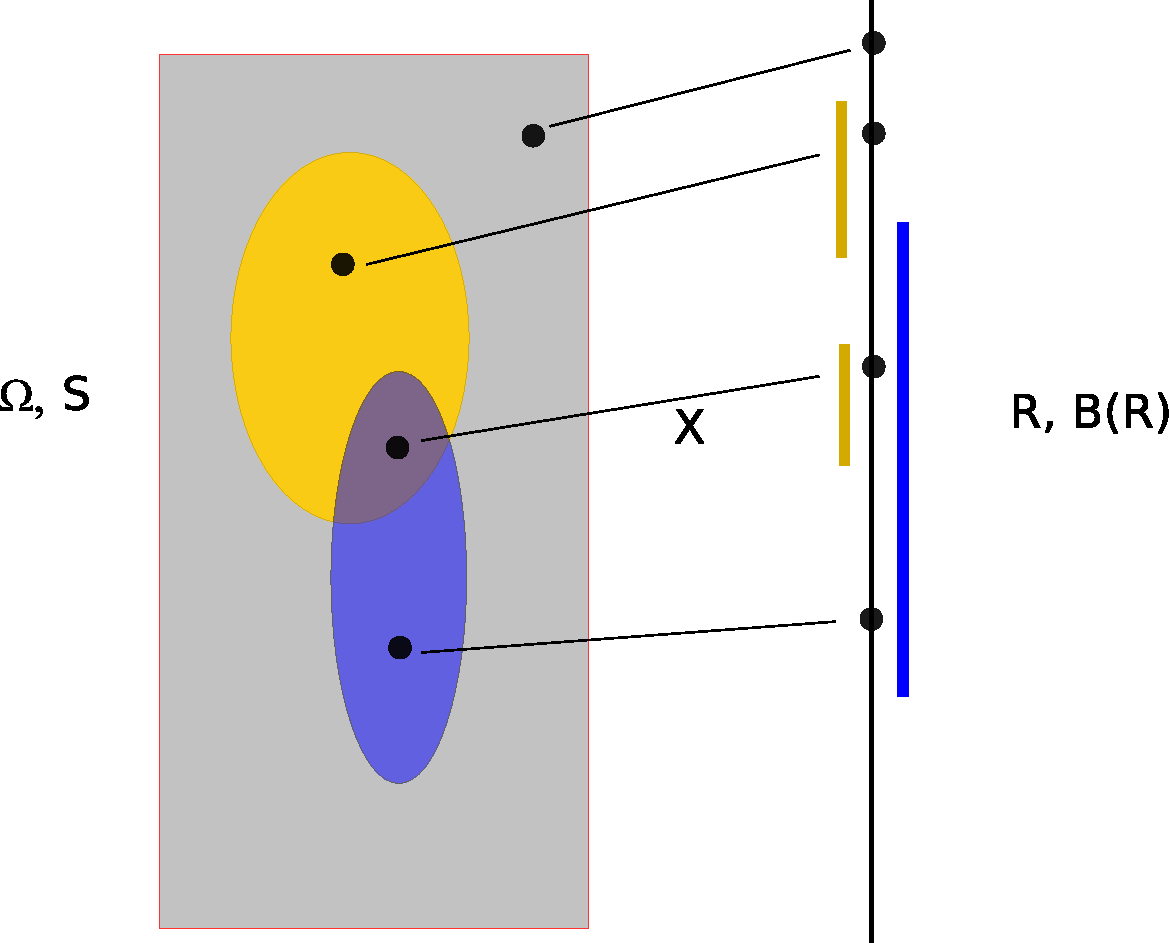
\includegraphics[scale=0.4]{nv.pdf}
\end{center}
\end{frame}


\begin{frame}{Náhodná veličina - definice}
\begin{definition}
 Nechť $(\Omega, \mathcal S, P)$ je pst. prostor.
 Pak náhodná veličina je zobrazení $X: \Omega \to \Real$, které je měřitelné,\\
 tj. vzor $X^{-1}(B)$ každé borelovské množiny $B\subset \Real$ je měřitelnou množinou $X^{-1}(B) \in \mathcal S$.
\end{definition}

\xskip
NV převádí lib. pst. prostor na prostor $(\Real, \mathcal B, \tilde P)$.\\

NV je určena \blue{distribuční funkcí} (DF): 
\[
   F_X(x) = \tilde P(X(\omega) < x) = P( X^{-1}\big(  (-\infty, x) \big)
\]
Dále nebudeme rozlišovat $\tilde P$ a $P$.
\end{frame}

\begin{frame}{Distribuční funkce}
Vlastnosti DF: 
\begin{enumerate}
 \item $0\le F(x) \le 1$
 \item $F$ je neklesající
 \item \[
  \lim_{x\to -\infty} F(x) = 0,\quad \lim_{x\to \infty} F(x) = 1
\]
 \item zleva spojítá 
\end{enumerate}

\begin{theorem}
  Pro každou funkci $F$ s vlastnostmi $1-4$ existuje náhodná veličina $X$, tak, že $F$ je její distribuční funkce.
\end{theorem}

\end{frame}



\begin{frame}{Diskrétní a spojitá rozdělení}
\blue{Diskrétní NV}\\
Pokud NV $X$ nabývá konečné nebo spočetné množiny hodnot $x_i$ a jejich psti jsou $p_i$, $\sum_i p_i =1$.\\
DF je skoková se skoky výšky $p_i$ v bodech $x_i$.

\xskip
\blue{Spojitá NV}
Pokud existuje nezáporná fce $f_X$ tak, že:
\[
   F_X(x) = \int_{-\infty}^x f_X(t) \dt
\]
$f_X$ se nazývá \blue{hustota pravděpodobnosti}. Platí $\int_{-\infty}^{\infty} f_X(x) = 1$.

DF spojité NV je spojitá fce. 

\end{frame}

\begin{frame}{Střední hodnota}
pro diskrétní náhodnou veličinu $X$:
\[
  EX = \sum_i x_i P(X = x_i) = \sum_i x_i p_i
\]
pro spojitou náhodnou veličinu $X$:
\[
  EX = \int_{-\infty}^{+\infty} xf_X(x) \d x
\]

\xskip
nemusí vždy existovat, např. $x_i = 2^n$, $p_i = 2^{-n}$\\
linearita: $E(aX+bY) = aEX + bEY$\\
střední hodnota transformované NV $Y = h(X)$: 
\[
 EY =  E h(X) = \int_{-\infty}^{+\infty} h(x) f_X(x) \d x
\]

\end{frame}

\begin{frame}{Momenty}
$r$-tý moment:
\[
 \mu'_r(X) = E(X^r)
\]
$r$-tý centrální moment: 
\[
 \mu_r(X) = E\big([X - EX]^r\big)
\] 
rozptyl $DX$, $\sigma^2$, $var(X)$: 
\begin{multline*}
  \mu_2(X) = DX = E( (X-EX)^2 ) = \\
E( X^2 + (EX)^2 - 2X EX) = E(X^2) - (EX)^2 = \mu'_2 - \mu'_1
\end{multline*}
směrodatná odchylka : $\sigma = \sqrt{\sigma^2}$\\
šikmost: $\alpha_3 = \mu_3/\sigma^3$\\
špičatost: $\alpha_4 = \mu_4/\sigma^4 -3$
\end{frame}

\begin{frame}{Kvantily}
Pro hodnotu $\alpha \in (0,1)$ najít bod $x$ takový, že $P(X < x) = \alpha$.  Definujeme
{\df kvantilovou funkci}:
\[
  F^{-1}(\alpha) = \inf\{x \where F_X(x)\ge\alpha\}
\]
označení: $x_\alpha$, $u_\alpha$; kavantil na hladině $\alpha$, $\alpha$-kvantil\\
medián $x_{0.5}$, kvartily,\dots

\vspace{2ex} POZOR: výběrový kvantil $Q_p$ se musí aproximovat. Např.
zaokrouhlením $Np$ k nejbližšímu indexu:
\[
  Q_p = x_i, \text{ kde } i = {\rm round}(Np)
\]
Jedná se tedy o odhad přesného kvantilu na základě realizací NV.



\end{frame}

\section{Příklady Diskrétních rozdělení}

\begin{frame}{Alternativní $Alt(p)$}
popis: počet úspěchů jednoho pokusu\\
př: vytažení prasklého vajíčka 

\xskip
hodnoty: $0, 1$\\
parametr: pravděpodobnost $p$

\xskip
$P( X=1 ) = p$\\
$EX = p$\\
$DX = p(1-p)$
\end{frame}

\begin{frame}{Binomické $Bi(n,p)$}
popis: počet úspěchů po $n$ pokusech\\
př: $k$ praských vajíček z $n$ vybraných, výběr s vracením

\xskip
hodnoty: $0, \dots, n$ \\
parametry: pst. $p$, počet pokusů $n$

\xskip
\[
 P(X=k) = \binom{n}{k}p^k(1-p)^{n-k};\quad 0\le k \le n
\]
$EX = np$\\
$DX = np(1-p)$

\xskip
$Alt(p) = Bi(1,p)$
\end{frame}

\begin{frame}{Hypergeometrické $H(N,M,n)$}
popis: počet úspěchů po $n$ pokusech pokud z $N$ je $M$ úspěchů\\
př: $k$ prasklých vajíček z $n$ vybraných, pokud jich je celkem $M$ prasklých z $N$\\
kontroly jakosti, výběr bez vracení

\xskip
hodnoty: $0, \dots, n$ \\
parametry: počet pokusů $n$, celkový počet prvků $N$, celkový počet prvků s valstností $M$

\xskip
\[
 P(X=k) = \frac{\text{příznivé}}{\text{všechny}}=
  \binom{M}{k}\binom{N-M}{n-k}\binom{N}{n}^{-1}
\]
\[
 P(k< n+M-N) = 1; \qquad  P(k> \min(M,n)) = 0
\]


$EX = \frac{nM}{N}$\\
$DX = \frac{nM}{N}\big(1-\frac{M}{N}\big)\big(\frac{N-n}{N-1}\big)$

$H(N,M,n) \approx Bi(n,M/N)$ pro velké hodnoty $N/n$
\end{frame}

\begin{frame}{Geometrické $G(p)$}
popis: počet výběrů do úspěchu (včetně)\\
př: kolik vytáhnu vajíček než najdu prasklé\\
počet provozních cyklů do poruchy

\xskip
hodnoty: $1, \dots, \infty$ \\
parametry: pravděpodobnost úspěchu $p$

\xskip
\[
 P(X=k) = (1-p)^{k-1}p
\]
$EX = \frac{1}{p}$\\
$DX = \frac{1-p}{p^2}$\\
\end{frame}

\begin{frame}{Negativní binomické $NB(k,p)$}
popis: počet výběrů do $k$ úspěchů (včetně)\\
př: kolik vytáhnu vajíček než najdu $k$ prasklých\\

\xskip
hodnoty: $k, \dots, \infty$ \\
parametry: pravděpodobnost úspěchu $p$

\xskip
\[
 P(X=n) = \binom{n-1}{k-1}(1-p)^{n-k}p^k
\]
$EX = \frac{k}{p}$\\
$DX = \frac{k(1-p)}{p^2}$\\
$NB(k,p)$ je jako součet $k$ veličin $G(p)$
\end{frame}

\begin{frame}{Poissonovo rozdělení}

{\df Poisonův proces}: počet výskytů náhodných událostí za časový interval, přičemž:
\begin{itemize}
 \item událostí je průměrně stále stejný počet $\lambda$ za jednotku času
 \item události jsou nezávislé
\end{itemize}
Př.: počet rozpadů jader za daný čas, počet defektů na délce materiálu

\xskip
hodnoty: $0,\dots,\infty$\\
parametry: hustota výskytu $\lambda$, doba $t$
\[
 P(X=k) = \frac{(\lambda t)^k e^{-\lambda t}}{k!}
\]
\end{frame}

\begin{frame}{Poissonovo rozdělení - odvození}

Rozdělíme interval $t$ na $n$ dílků a použijme $Bi(n, \lambda t/n)$ a provedeme limitu:
\begin{multline*}
 p_k = \lim_{n\to\infty} \frac{n!}{k!(n-k)!}\Big(\frac{\lambda t}{n}\Big)^k\Big(1-\frac{\lambda t}{n}\Big)^{n-k} =\\
 =\frac{(\lambda t)^k}{k!}\underbrace{\frac{n!}{n^k(n-k)!}}_{\to 1} \underbrace{\Big(1+\frac{-\lambda t}{n}\Big)^n}_{\to exp(-\lambda t)}
  \underbrace{\Big(1-\frac{\lambda t}{n}\Big)^{-k}}_{\to 1} 
\end{multline*}
\end{frame}

\begin{frame}{\dots odvození střední hodnoty a rozptylu}
Použitím rozvoje pro $\exp(\lambda t)$:
\[
  \sum_{k=0}^{\infty} \frac{(\lambda t)^k}{k!} e^{-\lambda t} = e^{-\lambda t} \sum_{k=0}^{\infty} \frac{(\lambda t)^k}{k!}  = e^{-\lambda t} e^{\lambda t} = 1
\]
Podobně odvodíme střední hodnotu:
\[
EX = \sum_{k=0}^{\infty} k \frac{(\lambda t)^k}{k!} e^{-\lambda t} =  \lambda t \sum_{k=0}^{\infty} \frac{(\lambda t)^{k-1}}{(k-1)!} e^{-\lambda t}=\lambda t
\]
\dots i rozptyl:
\begin{multline*}
DX = \sum_{k=0}^{\infty} (k^2 - (EX)^2)p_k = \sum_{k=0}^{\infty} k(k-1)p_k + kp_k - (\lambda t)^2 p_k = \\
=(\lambda t)^2 +(\lambda t) - (\lambda t)^2 = \lambda t 
\end{multline*}
  
\end{frame}

\end{document}


